\documentclass{article}
\usepackage[utf8]{inputenc}
\usepackage[russian]{babel}
\usepackage[left=2cm,right=2cm,
top=2cm,bottom=2cm,bindingoffset=0cm]{geometry}
\usepackage{graphicx}
\usepackage{amsmath}
\usepackage{float}
\usepackage{listings}
\usepackage{url,textcomp}
\date{2019 г.}
\author{Кондратенко Федор, гр 13632/1}
\setlength{\parindent}{0pt}
\setlength{\parskip}{5pt plus 2pt minus 1pt}
\frenchspacing
\title{Отчет по заданию №8}
\begin{document}
	\maketitle
	\paragraph*{Убиквитин\\}
	Гидрофобные остатки располагаются внутри молекулы, что дает убиквитину устойчивость к растворителям.\\
	\begin{figure}[H]
		\centering
		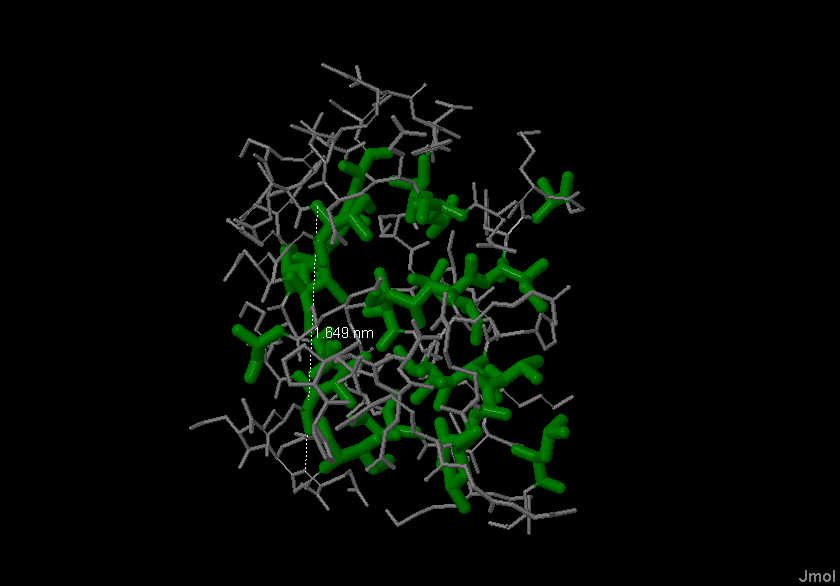
\includegraphics[width=0.7\linewidth]{ubi}
		\caption{Молекула убиквитина}
		\label{fig:ubi}
	\end{figure}
	
	Вид с другого ракурса:
	\begin{figure}[H]
		\centering
		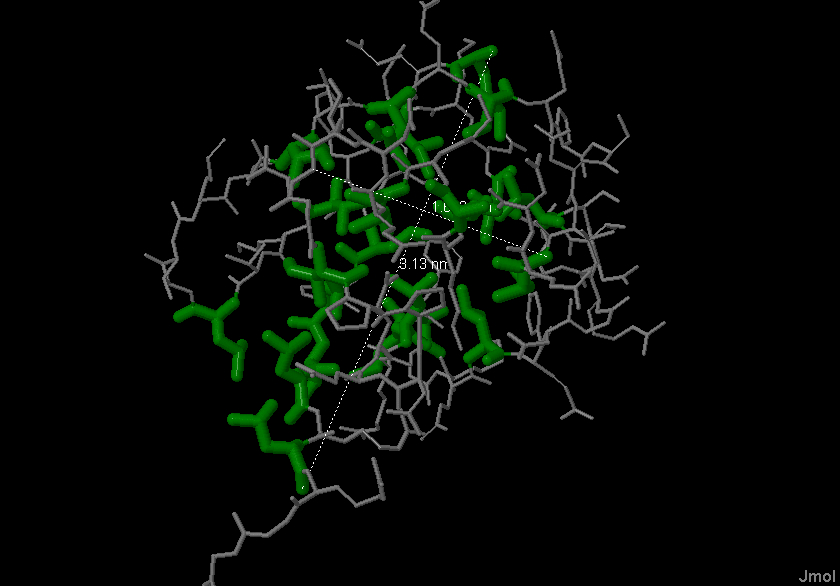
\includegraphics[width=0.7\linewidth]{ubi2}
		\caption{Вид с другого ракурса и с указанным размером}
		\label{fig:ubi2}
	\end{figure}
	Размер молекулы убиквитина 3.13 нм.
	\paragraph*{Аспирин\\}
	Аспирин не содержит гидрофобных остатков, соответственно, не подвержен влиянию растворителей.
	\begin{figure}[H]
		\centering
		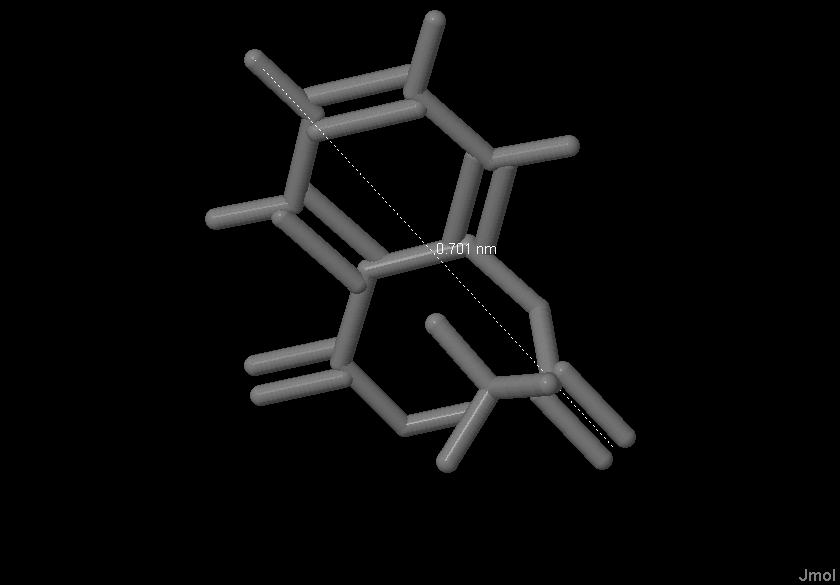
\includegraphics[width=0.7\linewidth]{aspirin}
		\caption{Аспирин}
		\label{fig:aspirin}
	\end{figure}
	Размеры молекулы -- 0.701 нм.
	\paragraph*{Гемагглютинин вируса гриппа H5N1\\}
	5-й известный тип гемагглютинина:
	\begin{figure}[H]
		\centering
		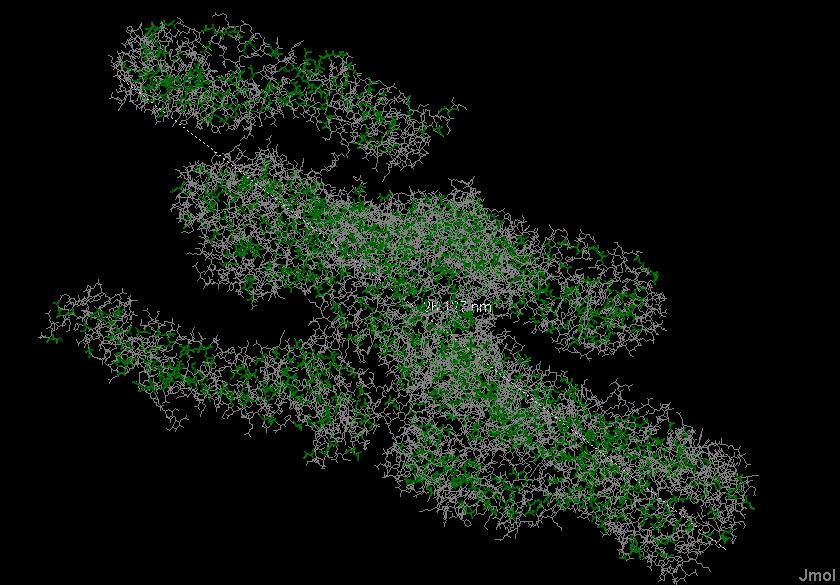
\includegraphics[width=0.7\linewidth]{h5n126-127}
		\caption{Гемагглютинин вируса H5Nq}
		\label{fig:h5n126-127}
	\end{figure}
	Размер молекулы -- 26.127 нм.
	\paragraph*{Белок с идентификатором 2DHB\\}
	Размер молекулы -- 4.763 нм.
	\begin{figure}[H]
		\centering
		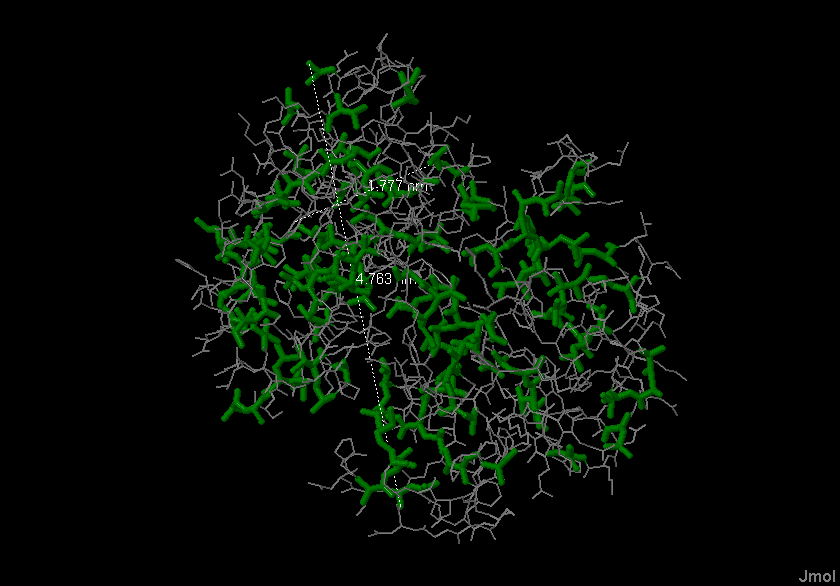
\includegraphics[width=0.7\linewidth]{2dhb}
		\caption{2DHB}
		\label{fig:2dhb}
	\end{figure}
	\paragraph*{Гемоглобин\\}
	Гемоглобин, идентификатор 4hhb. Представляет собой кольцо, гидрофобные остатки идут, в большинстве, по внутреннему радиусу.
	\begin{figure}[H]
		\centering
		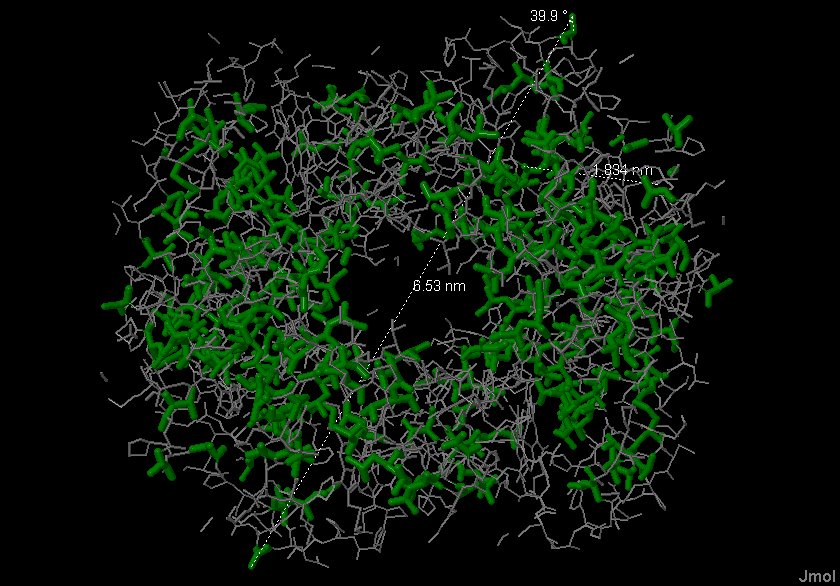
\includegraphics[width=0.7\linewidth]{4hhb}
		\caption{4hhb}
		\label{fig:4hhb}
	\end{figure}
	Внешний радиус -- 6.53 нм.
	\paragraph*{Белок 1vqx \\}
	Гидрофобные остатки четко структурированны, находятся в трех больших группах на концах молекулы.
	\begin{figure}[H]
		\centering
		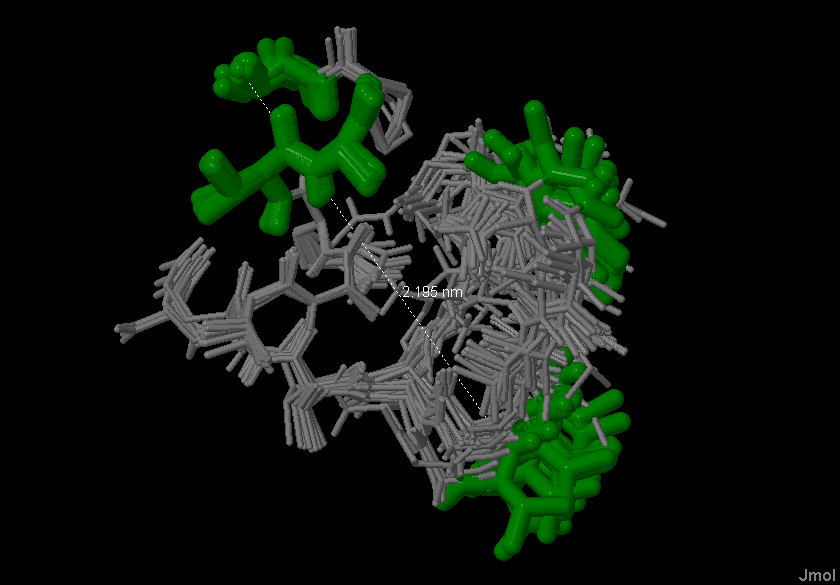
\includegraphics[width=0.68\linewidth]{1vqx}
		\caption{1vqx}
		\label{fig:1vqx}
	\end{figure}
	Размер молекулы -- 2.195 нм.
\end{document}